\documentclass[10pt,onecolumn]{article}
\usepackage[utf8]{inputenc}
\usepackage[english]{babel}
\usepackage[T1]{fontenc}
\usepackage{lmodern}
\usepackage{multicol}
\usepackage{amsmath}
\usepackage{amssymb}
\usepackage{mathrsfs}
\usepackage{float}
\usepackage[section]{placeins}
\usepackage{graphbox}
\usepackage{pbox}
\usepackage{longtable}
\usepackage{nicefrac}
\usepackage[margin=1.5cm]{geometry}

\DeclareMathSizes{10}{10}{10}{10}

% --- 
% Beginning of document
% ---
\begin{document}
%{%<- was never closed
	\setlength{\parindent}{0pt}
\part{Basic Properties \& Facts}

% --- 
% Arithmetic section
% ---
\section{Arithmetic}
\begin{center}
{\renewcommand{\arraystretch}{2}
\begin{tabular}[c]{| c | c | c | c | c}
\hline
$\frac{ab + ac}{a} = b + c, a\neq 0 $ & 
$\frac{a}{b} + \frac{c}{d} = \frac{ad + bc}{bd}$ & 
$\frac{a - b}{c - d} = \frac{b - a}{d - c}$ &
$\frac{a + b}{c} = \frac{a}{c} + \frac{b}{c}$ \\
\hline
$\nicefrac{\frac{a}{b}}{\frac{c}{d}} = \frac{ad}{bc}$ & 
$\frac{a}{b} - \frac{c}{d} = \frac{ad - bc}{bd}$ & 
$a \frac{b}{c} = \frac{ab}{c}$ &
$ab + ac = a(b+c) $ \\
\hline
\end{tabular}}
\end{center}

\subsection{Common arithmetic errors}

\begin{center}
{\renewcommand{\arraystretch}{2}
\begin{tabular}{| c | c | }
\hline
Error & Reason/correction/justification/example \\
\hline
$\frac{2}{0} \neq 0 $ and $\frac{2}{0} \neq 2 $ & Division by zero is undefined! \\
\hline
$\frac{a}{b + c} \neq \frac{a}{b} + \frac{b}{c}$ & $\frac{1}{2} = \frac{1}{1 + 1} \neq \frac{1}{1} + \frac{1}{1} = 2$  \\
\hline
$\frac{1}{x^2 + x^3} \neq x^{-2} + x^{-3}$ & A more complex version of the previous error.  \\
\hline
$\frac{\not a + bx}{\not a} \neq 1 + bx$  & $\frac{a + bx}{a} = \frac{a}{a} + \frac{bx}{a} = 1 + \frac{bx}{a}$\\
\hline
$\frac{a}{\frac{b}{c}} \neq \frac{ab}{c}$ & $\frac{a}{\frac{b}{c}} = \frac{\frac{a}{1}}{\frac{b}{c}} = \frac{a}{1} \frac{c}{b} = \frac{ac}{b}$ \\
\hline
$\frac{\frac{a}{b}}{c} \neq \frac{ac}{b}$ & $\frac{\frac{a}{b}}{c} = \frac{\frac{a}{b}}{\frac{c}{1}} = \frac{a}{b} \frac{1}{c} = \frac{a}{bc}$ \\
\hline
$-a(x-1) \neq -ax - a$ & $-a(x-1) \neq -ax + a$  \\
\hline


\end{tabular}}
\end{center}

% --- 
% Exponent section
% ---
\section{Exponent}
\begin{center}
{\renewcommand{\arraystretch}{2}
\begin{tabular}[c]{| c | c | c | c | c |}
\hline
$a^n a^m = a^{n+m} $ & 
$(a^n)^m = a^{nm} $ & 
$(ab)^n = a^n b^n$ & 
$a^{-n} = \frac{1}{a^n}$ & 
$(\frac{a}{b})^{-n} = (\frac{b}{a})^{n} = \frac{b^n}{a^n} $ \\
\hline
$\frac{a^n}{a^m} = a^{n-m} = \frac{1}{a^{m-n}}$ & 
$a^0 = 1, a \neq 0 $ & 
$(\frac{a}{b})^n = \frac{a^n}{b^n}$ & 
$\frac{1}{a^{-n}} = a^n$ & 
$a^\frac{n}{m} = (a^\frac{1}{m})^n = (a^n)^\frac{1}{m}$ \\
\hline
\end{tabular}}
\end{center}

\subsection{Common exponent errors}

\begin{center}
{\renewcommand{\arraystretch}{2}
\begin{tabular}{| c | l | }
\hline
Error & Reason/correction/justification/example \\
\hline
$-3^2 \neq 9$ & $-3^2 = -9$, $(-3^2) = 9$ Watch parenthesis !  \\
\hline
$(x^2)^3 \neq x^5$ & $(x^2)^3 = x^6$   \\
\hline
$(x + a)^2 \neq x^2 + a^2$ & $(x + a)^2 = (x + a)(x + a) = x^2 + 2ax + a^2 $ \\
\hline
$2(x+1)^2 \neq (2x + 2)^2 $ & $2(x + 1)^2 = 2(x^2 + 2x + 1) = 2x^2 + 4x + 2$, \\ 
& $(2x^2 + 2)^2 = 4x^2 +8x + 4 $ \\
\hline
$(2x + 2)^2 \neq 2(x + 1)^2$ & No factor out a constant if there is a power on the parenthesis! \\
\hline
$(x + a)^n \neq x^n + a^n$ and $\sqrt[n]{x + a} \neq \sqrt[n]{x} + \sqrt[n]{a}$ & More general versions of previous three errors \\
\hline
\end{tabular}}
\end{center}


% --- 
% Radicals section
% ---
\section{Radicals}
\begin{center}
{\renewcommand{\arraystretch}{2}
\begin{tabular}[c]{| c | c | c |}
\hline
$\sqrt[n]{a^m} = a^{\frac{m}{n}}$ &
$\sqrt[m]{\sqrt[n]{a}} = \sqrt[mn]{a}$ &
$\sqrt[n]{a^n} = a, \text{if n is odd} $ \\
\hline
$\sqrt[n]{a^n} = |a|, \text{if n is even} $ &
$\sqrt[n]{ab} = \sqrt[n]{a}\sqrt[n]{b}$ &
$\sqrt[n]{\frac{a}{b}} = \frac{\sqrt[n]{a}}{\sqrt[n]{b}}$ \\
\hline
\end{tabular}}
\end{center}

\subsection{Square Root property}
If $ x^2 = p $ then $ x = \pm \sqrt{p}$

\subsection{Common radicals errors}

\begin{center}
{\renewcommand{\arraystretch}{2}
\begin{tabular}{| c | c | }
\hline
Error & Reason/correction/justification/example \\
\hline
$\sqrt{x^2 + a^2} \neq x + a $ & $5 = \sqrt{25} = \sqrt{3^2 + 4^2} \neq \sqrt{3^2} + \sqrt{4^2} = 3 + 4 = 7 $ \\
\hline
$\sqrt{x + a} \neq \sqrt{x} + \sqrt{a} $ & See previous error \\
\hline
$\sqrt{-x^2 + a^2} \neq -\sqrt{x^2 + a^2} $ & $\sqrt{-x^2 + a^2} = (-x^2 + a^2)^\frac{1}{2}$ \\
\hline
\end{tabular}}
\end{center}

% --- 
% Inequalities section
% ---
\section{Inequalities}
If a < b then a + c < b + c and a - c < b - c \\\\
If a < b and c > 0 then ac < bc and $\frac{a}{c} < \frac{b}{c}$ \\\\
If a < b and c < 0 then ac > bc and $\frac{a}{c} > \frac{b}{c}$ \\\\

\text{When both sides a multiplied by a negative, the inequality's side must be changed} \\
\begin{align*}
-a &< b \\
a &> -b
\end{align*}

\text{A constant/variable must be moved on all sides of an inequality} \\
\begin{align*}
a 	&< x + b 	< c \\
a - b 	&< x 		< c - b \\ 
\\
a &< x*b < c \\
\frac{a}{b}  &< x < \frac{c}{b} \\
\end{align*}

\pagebreak
% --- 
% Absolute value section
% ---
\section{Absolute value}
\begin{center}
{\renewcommand{\arraystretch}{2}
\begin{tabular}{| c | c | c |}
\hline
$\left|a\right| = a $, if $a \ge 0$, -a if $a < 0$ &
$\left|a\right| \ge 0 $ &
$\left|ab\right| = \left|a\right|\left|b\right| $ \\
\hline
$\left|a+b\right| \le \left|a\right| + \left|b\right|$ &
$\left|-a\right| = \left|a\right| $ &
$\left|\frac{a}{b}\right| = \frac{\left|a\right|}{\left|b\right|} $ \\
\hline
\end{tabular}}
\end{center}

% --- 
% Absolute value section
% ---
\section{Absolute value and inequalities}
\begin{center}
{\renewcommand{\arraystretch}{2}
\begin{tabular}{| c | c |}
\hline
$\left|p\right| = b $ & $p = -b $ or $ p = b $ \\
\hline
$\left|p\right| < b $ & $-b < p < b $ \\
\hline
$\left|p\right| > b $ & $p < -b $ or $ p > b $ \\
\hline
\end{tabular}}
\end{center}

% --- 
% Complex numbers section
% ---
\section{Complex numbers}
\begin{center}
{\renewcommand{\arraystretch}{2}
\begin{tabular}{| c | c |}
\hline
$\sqrt{-a} = i\sqrt{a}, a \ge 0 $ &
$(a + bi) + (c + di) = a+ c + (b + d)i$ \\
\hline
$(a + bi) - (c + di) = a - c + (b - d)i $ &
$(a + bi)(c - di) = ac - bd + (ad + bc)i$ \\
\hline
$(a + bi)(a - bi) = a^2 + b^2 $ &
$\left|a + bi\right| = \sqrt{a^2 + b^2} $ Complex Modulus \\
\hline
$\bar{(a + bi)}(a + bi) = \left|a + bi\right|^2 $ &
$\bar{(a + bi)} = a - bi $ Complex Conjugate \\
\hline
\end{tabular}}
\end{center}

\subsection{Main values of $i $}
\begin{align*}
i &= \sqrt{-1} \\
i^2 &= -1 \\
i^3 &= -i \\
i^4 &= 1 
\end{align*}

% --- 
% Logarithms and Log properties section
% ---
\section{Logarithms and Log properties}
\subsection{Definition and special Logarithms}
$y = \log_b x$ is equivalent to $x = b^y$ \\
$ln x = \log_e x $ (Natural Log) \\
$\log x = \log_{10} x $ (Common Log) \\
The domain of $\log_b x$ is $x > 0$ 

\subsection{Logarithms properties}
\begin{center}
{\renewcommand{\arraystretch}{2}
\begin{tabular}{| c | c | c | c |}
\hline
$\log_b b = 1 $ &
$\log_b 1 = 0 $ &
$\log_b b^x = x $ &
$b^{\log_b x} = x $ \\
\hline
$\log_b (x^r) = r \cdot \log_b x $ &
$\log_b (xy) = \log_b x + \log_b y $ &
$\log_b (\frac{x}{y}) = \log_b x - \log_b y$ &
$\log_b x = \frac{\log_d(x)}{\log_d(b)} $ \\
\hline
\end{tabular}}
\end{center}

% --- 
% Factoring and Solving section
% ---
\section{Factoring and Expanding}
\begin{align*}
x^2 - a^2  & =  (x+a)(x-a) \\
(x+a)^2  & =  x^2 + 2ax + a^2  \\
(x-a)^2  & =  x^2 - 2ax + a^2  \\
(x+a)(x+b)  & =  x^2 + (a+b)x + ab  \\
(x+a)^3  & = x^3 + 3ax^2 + 3a^{2}x + a^3 \\
(x-a)^3  & = x^3 - 3ax^2 + 3a^{2}x - a^3 \\
x^3 + a^3 & = (x+a)(x^2 - ax + a^2) \\
x^3 - a^3  & = (x-a)(x^2 + ax + a^2) \\
x^{2n} - a^{2n}  & = (x^n - a^n)(x^n + a^n) \\
\end{align*}


% --- 
% Quadratic formula section
% ---
\section{Quadratic formula}
Find the roots of a quadratic equation : \\
\begin{align*}
ax^2 + bx + c = 0; a \neq 0  \\
x = \frac{-b \pm \sqrt{b^2 - 4ac}}{2a} 
\end{align*}

\pagebreak
% --- 
% Completing the square section
% ---
\section{Completing the square}
Solve : \\
\begin{align*}
2x^2 - 6x - 10 = 0
\end{align*}
(1) Divide the coefficient of the $x^2$ \\
\begin{align*}
x^2 -3x - 5
\end{align*}
(2) Move the constant to the other side \\
\begin{align*}
x^2 - 3x = 5 
\end{align*}
(3) Take half the coef. of x, square it and add it to both sides \\
\begin{align*}
x^2 - 3x + \bigg(\frac{-3}{2}\Big)^2 = 5 + \left(\frac{-3}{2}\right)^2
\end{align*}
(4) Factor the left side \\
\begin{align*}
\bigg(x - \frac{3}{2}\bigg)^2 = \frac{29}{4}
\end{align*}
(5) Use square root property \\
\begin{align*}
x - \frac{3}{2} = \pm \sqrt{\frac{29}{4}}
\end{align*}
(6) Solve for x \\
\begin{align*}
x = \frac{3}{2} \pm \frac{\sqrt{29}}{2}
\end{align*}
\pagebreak

\part{Functions and Graphs}

% --- 
% Distance formula section
% ---
\section{Distance formula}
If $P_1 = (x_1, y_1) $ and $P_2 = (x_2, y_2)$ are two points. The distance between them is equal to : \\
\begin{align*}
d(P_1, P_2) = \sqrt{(x_2 - x_1)^2 + (y_2 - y_1)^2}
\end{align*}

% --- 
% Constant Function
% ---
\section{Constant function}
$y = a$ or $f(x) = a $ \\ 
Graph is a horizontal line passing through the point (0,a). \\
Domain $= \mathbb{R}$; Range = $\{f \in \mathbb{R} \colon f = a\} $ 

% --- 
% Linear Function
% ---
\section{Linear function}
\begin{table}[H]
\begin{center}
\begin{tabular}{|c|l|}
\hline
\multicolumn{1}{|c|}{Graph} & \multicolumn{1}{c|}{Information about f(x)} \\
\hline

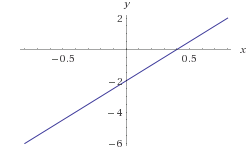
\includegraphics[align=c]{graph_linear_function.png}
&
\pbox{15cm}
{
  $f(x) = mx + b $ \\
  Graph is a line with point (0,b) \\
  Slope $m$.%Needs to be a variable here as well
  Example : $f(x) = 5x - 2 $ \\
} \\
\hline
\end{tabular}
\end{center}
\end{table}

Slope : slope of the line containing the two points $(x_1, y_1)$ and $(x_2, y_2)$ : \\
\begin{align*}
	\frac{y_2 - y_1}{x_2 - x_1} = \frac{\text{rise}}{\text{run}} \\%%%JB words are text
\end{align*}

Slope - intercept form : the equation of the line with slope $m$ and $y$-intercept $(0, b)$ is : \\%also math
\begin{align*}
y = mx + b 
\end{align*}

Point - Slope from : the equation of the line with slope m and passing through the point $(x_1, y_1)$ is : 
\begin{align*}
y - y_1 =  m(x - x_1)  \\
\end{align*}

Find x-intercept, set equation equal to 0 and solve for x : \\
\begin{align*}
0 & = 5x - 2 \\
\frac{2}{5} & = x \\
\end{align*}

Find y-intercept; set x equal to 0 and solve for y : \\
\begin{align*}
y & = 5(0) - 2 \\
y & = -2 \\
\end{align*}

% --- 
% Quadratic Function
% ---
\section{Parabola/Quadratic function}
\begin{center}
\begin{longtable}{|c|l|}
\hline
\multicolumn{1}{|c|}{Graph} & \multicolumn{1}{c|}{Information about f(x)} \\
\hline

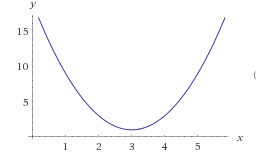
\includegraphics[align=c]{graph_parabola_function_1_up.png}
&
\pbox{15cm}
{
  $f(x) = a(x - h)^2 + k $ \\
  Parabola that opens up if $a > 0$ or down if $a < 0$ \\
  Vertex at (h, k) \\
  Example : $f(x) = 2(x - 3)^2 + 1 $ \\
} \\
\hline

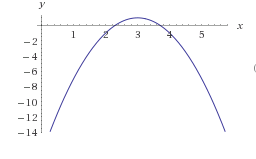
\includegraphics[align=c]{graph_parabola_function_1_down.png}
&
\pbox{15cm}
{
  $f(x) = a(x - h)^2 + k $ \\
  Parabola that opens up if $a > 0$ or down if $a < 0$ \\
  Vertex at (h, k) \\
  Example : $f(x) = -2(x - 3)^2 + 1 $ \\
} \\
\hline

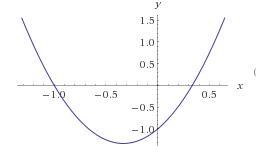
\includegraphics[align=c]{graph_parabola_function_2_up.png}
&
\pbox{15cm}
{
  $f(x) = ax^2 + bx + c$ \\
  Parabola that opens up if $a > 0$ or down if $a < 0$ \\
  Vertex at ($\frac{-b}{2a}, f - \frac{b}{2a} $) \\
  Example : $f(x) = 3x^2 + 2x - 1$ \\
} \\
\hline

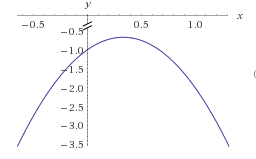
\includegraphics[align=c]{graph_parabola_function_2_down.png}
&
\pbox{15cm}
{
  $f(x) = ax^2 + bx + c$ \\
  Parabola that opens up if $a > 0$ or down if $a < 0$ \\
  Vertex at ($\frac{-b}{2a}, f - \frac{b}{2a} $) \\
  Example : $f(x) = -3x^2 + 2x - 1$ \\
} \\
\hline

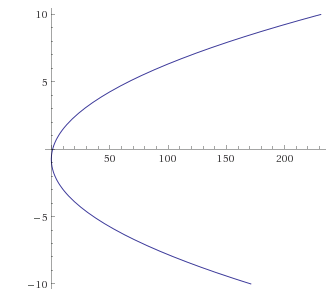
\includegraphics[align=c]{graph_parabola_function_3_right.png}
&
\pbox{15cm}
{
  $g(y) = ay^2 + by + c $ \\
  Parabola that opens right if $a > 0$ or left  if $a < 0$ \\
  Vertex at ($\frac{-b}{2a}, g - \frac{b}{2a} $) \\
  Example : $g(y) = 2y^2 + 3y + 1 $ \\
} \\
\hline

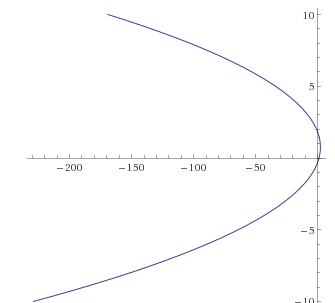
\includegraphics[align=c]{graph_parabola_function_3_left.png}
&
\pbox{15cm}
{
  $g(y) = ay^2 + by + c $ \\
  Parabola that opens right if $a > 0$ or left  if $a < 0$ \\
  Vertex at ($\frac{-b}{2a}, g - \frac{b}{2a} $) \\
  Example : $g(y) = -2y^2 + 3y + 1 $ \\
} \\
\hline

\end{longtable}
\end{center}

% --- 
% Circle Function
% ---
\section{Circle}
\begin{table}[H]
\begin{center}
\begin{tabular}{|c|l|}
\hline
\multicolumn{1}{|c|}{Graph} & \multicolumn{1}{c|}{Information about f(x)} \\
\hline

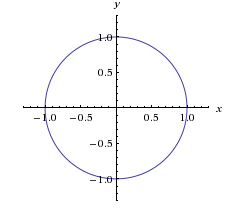
\includegraphics[align=c]{graph_circle.png}
&
\pbox{15cm}
{
  $(x - h)^2 + (y - k)^2 = r^2  $ \\
  Circle with radius r and center (h, k) \\
  Example : $x^2 + y^2 = 1 $ \\
} \\
\hline
\end{tabular}
\end{center}
\end{table}


% --- 
% Ellipse Function
% ---
\section{Ellipse}
\begin{table}[H]
\begin{center}
\begin{tabular}{|c|l|}
\hline
\multicolumn{1}{|c|}{Graph} & \multicolumn{1}{c|}{Information about f(x)} \\
\hline

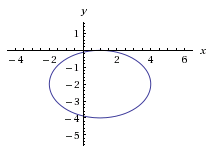
\includegraphics[align=c]{graph_ellipse.png}
&
\pbox{15cm}
{
  $\frac{(x - h)^2}{a^2} + \frac{(y - k)^2}{b^2} = 1$ \\
  Graph is an ellipse with center (h, k). \\
  Vertices \emph{a} units right/left from the center \\
  Vertices \emph{b} units up/down from the center \\
  Example : $\frac{(x-1)^2}{3^2} + \frac{(y+2)^2}{2^2} = 1$) \\
} \\
\hline
\end{tabular}
\end{center}
\end{table}

% --- 
% Hyperbola Function
% ---
\section{Hyperbola}
\begin{table}[H]
\begin{center}
\begin{tabular}{|c|l|}
\hline
\multicolumn{1}{|c|}{Graph} & \multicolumn{1}{c|}{Information about f(x)} \\
\hline

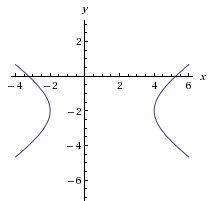
\includegraphics[align=c]{graph_hyperbola_1.png}
&
\pbox{15cm}
{
  $\frac{(x - h)^2}{a^2} - \frac{(y - k)^2}{b^2} = 1$ \\
  Hyperbola that opens left and right \\
  Center at (h, k) \\ 
  Vertices \emph{a} units left/right of center \\
  Asymptotes pass through center with slope $\pm \frac{b}{a}$ \\
  Example : $\frac{(x-1)^2}{3^2} - \frac{(y+2)^2}{2^2} = 1 $ \\
} \\
\hline 

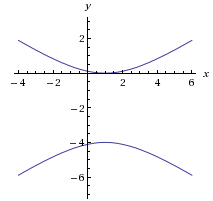
\includegraphics[align=c]{graph_hyperbola_2.png}
&
\pbox{15cm}
{
  $\frac{(y - k)^2}{b^2} - \frac{(x - h)^2}{a^2} = 1$ \\
  Hyperbola that opens up and down \\
  Center at (h, k) \\
  Vertices \emph{b} units up/down of center \\ 
  Asymptotes pass through center with slope $\pm \frac{b}{a}$ \\
  Example : $\frac{(y+2)^2}{2^2} + \frac{(x-1)^2}{3^2} = 1$ \\
} \\
\hline
\end{tabular}
\end{center}
\end{table}

% --- 
% Main/Common Functions
% ---
\section{Main/Common functions}

\begin{center}
\begin{longtable}{c|c}
\hline
\multicolumn{1}{|c|}{Graph} & \multicolumn{1}{c|}{Information about f(x)} \\
\hline

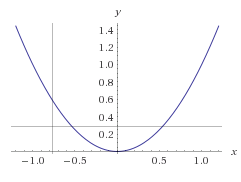
\includegraphics[align=c]{graph_x_2.png}
&
\pbox{15cm}
{
  $f(x) = x^2 $ \\
  Domain : $= \mathbb{R}$ \\
  Range : $\{y \in \mathbb{R} \colon y \ge 0 \} $ \\
  Parity : even\\
  Root at x = 0
} \\


\hline
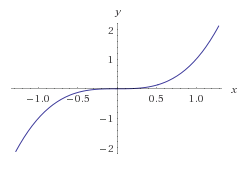
\includegraphics[align=c]{graph_x_3.png}
&
\pbox{15cm}
{
  $f(x) = x^3 $ \\
  Domain : $\mathbb{R}$ \\
  Range : $\mathbb{R}$ \\
  Parity : odd \\
  Root at x = 0
} \\


\hline
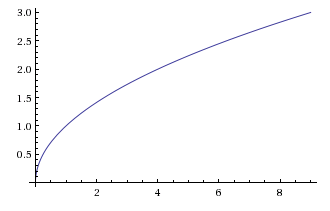
\includegraphics[align=c]{graph_sqrt_x.png}
&
\pbox{15cm}
{
  $f(x) = \sqrt(x) $\\
  Domain : $x \in \mathbb{R} \colon x \ge 0 $ \\
  Range : $y \in \mathbb{R} \colon y \ge 0 $ \\
  Root at x = 0
} \\


\hline
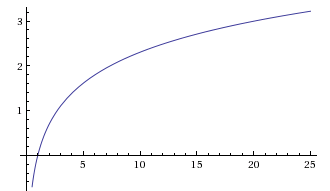
\includegraphics[align=c]{graph_ln.png}
&
\pbox{15cm}
{
  $f(x) = \ln(x) $\\
  Domain : $x \in \mathbb{R} \colon x > 0 $ \\
  Range : $ \mathbb{R} $ \\
  Root at x = 1
} \\


\hline
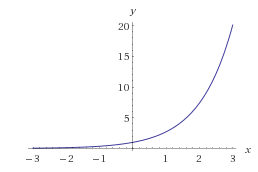
\includegraphics[align=c]{graph_e_x.png}
&
\pbox{15cm}
{
  $f(x) = e^x $\\
  Domain : $\mathbb{R}$ \\
  Range : $y \in \mathbb{R} \colon y > 0 $ \\
  Root : none
} \\

\hline
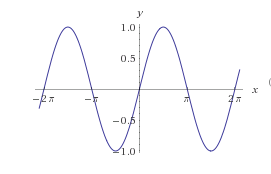
\includegraphics[align=c]{graph_sin.png}
&
\pbox{15cm}
{
  $f(x) = sin(x) $\\
  Domain : $\mathbb{R}$ \\
  Range : $y \in \mathbb{R} \colon -1 \le y \le 1 $ \\
  Root : $x = \pi n, n \in \mathbb{Z}$\\
  Periodicity : in x with period $2\pi$ \\
  Parity : odd
} \\


\hline
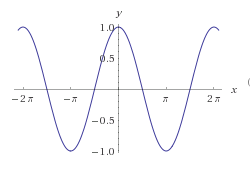
\includegraphics[align=c]{graph_cos.png}
&
\pbox{15cm}
{
  $f(x) = cos(x)$\\
  Domain : $\mathbb{R}$ \\
  Range : $y \in \mathbb{R} \colon -1 \le y \le 1 $ \\
  Root : $x = \pi n - \frac{\pi}{2}, n \in \mathbb{Z}$\\
  Periodicity : in x with period $2\pi$ \\
  Parity : even
} \\


\hline
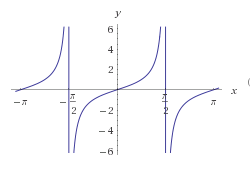
\includegraphics[align=c]{graph_tan.png}
&
\pbox{15cm}
{
  $f(x) = tan(x)$\\
  Domain : $x \in \mathbb{R} : \pi(n + \frac{1}{2}) < x < \pi(n + \frac{3}{2})$ \\
  and $n \in \mathbb{Z}$ \\
  Range : $\mathbb{R}$ \\
  Root : $x = \pi n, n \in \mathbb{Z}$\\
  Periodicity : in x with period $\pi$ \\
  Parity : even
} \\


\hline
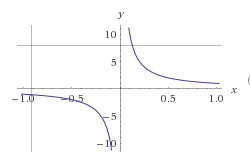
\includegraphics[align=c]{graph_1_over_x.png}
&
\pbox{15cm}
{
$\frac{1}{x}$\\
  Domain : $x \in \mathbb{R} : x \ne 0$ \\
  Range : $y \in \mathbb{R} : y \ne 0$ \\
  Root : none\\
  Parity : odd
} \\


\hline
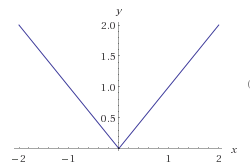
\includegraphics[align=c]{graph_abs_x.png}
&
\pbox{15cm}
{
$\left|x\right|$\\
  Domain : $\mathbb{R}$ \\
  Range : $y \in \mathbb{R} : y \ge 0$ \\
  Root at x = 0
} \\

\hline
\end{longtable}
\end{center}
% --- 
% End of document
% ---
\end{document}
